\documentclass{report}

\usepackage{fullpage}
\usepackage[skip=4pt]{caption} % ``skip'' sets the spacing between the figure and the caption.
\usepackage{pgfplots}   % Needed for plotting
\usepackage{amsmath}    % Allows for piecewise functions using the ``cases'' construct
\usepackage{graphics}   % Allows figures in the document.
\graphicspath{{img/}}
\usepackage{multicol}   % Used for two column lists

\usepackage{tikz}
\usetikzlibrary{matrix, positioning, calc, shadows}
\usepackage{xcolor}

%\usepackage[hidelinks]{hyperref}   % Make the cross references clickable hyperlinks
%\usepackage[bottom]{footmisc} % Prevents the table going below the footnote

% Set up page formatting
\usepackage{fancyhdr} % Used for every page footer and title.
\pagestyle{fancy}
\fancyhf{} % Clears both the header and footer
\renewcommand{\headrulewidth}{0pt} % Eliminates line at the top of the page.
\fancyfoot[LO]{CMPS242 \textendash{} Homework \#5} % Left
\fancyfoot[CO]{\thepage} % Center
\fancyfoot[RO]{Sherman \& Hammoudeh} %Right

\renewcommand\thesection{\arabic{section}} % Prevent chapter number in section number.

% Change interline spacing.
\renewcommand{\baselinestretch}{1.1}
\newcommand{\norm}[1]{\left\lVert#1\right\rVert}


\title{\textbf{CMPS242 Homework \#5 \textendash{} \\Neural Network Tweet Classification}}
\author{Benjamin Sherman \\~\\ \& \\~\\ Zayd Hammoudeh \\~\\ \textbf{Team Name}: ``Who Farted?''}
\date{} % Remove date on cover page


\begin{document}
  \maketitle
  
  \suppressfloats % No images on the first page.
  \section{Homework Objective}
  
  Develop a long short term memory-based (LSTM) neural network that classifies tweets as being sent by either Hillary Clinton (@HillaryClinton) or Donald Trump (@realDonaldTrump).
  
  \section{Dataset Overview}
  
  The dataset is a comma-separated list of tweets from either @HillaryClinton or @realDonaldTrump.  No additional information is provided beyond the tweet's text and potentially the class label.  The training set consists of 4,743~tweets while the test set has 1,701~unlabeled tweets.
   
  \section{Tweet Text Preprocessor}\label{sec:textPreprocessor}
  
  Since an LSTM is a recursive neural network, it can rely on both vocabulary and contextual information to perform classification.  Extensive text preprocessing has the potential to destroy subtle textual information.  As such, we performed very minimal text manipulation beyond vectorization.  For example, we left all stop words in place.  We removed some of the punctuation but left hashtags~(\#) and exclamation points as we theorized that they may be part of a specific user's unique tweet ``signature.''  This results in a vocabulary of approximately eleven thousand words; it should be noted that a small percentage of this vocabulary is gibberish, one-off, shortened URLs.  We believe that with additional effort, we may be able to derive useful information from these URLs, but we leave that as a future exercise.
   
  \section{Classifier Structure}
  
  At a minimum, this homework's LSTM classifier must have the structure shown in Figure~\ref{fig:completeLstmClassifer}.  There are four primary components, namely the embedding matrix, one-hot vector, long short-term memory network, and feed-forward network,which are described in the following subsections.
  
  \begin{figure}
    \centering
    \tikzset{
      sigmoid/.style={path picture= {
          \begin{scope}[x=1pt,y=10pt]
            \draw plot[domain=-6:6] (\x,{1/(1 + exp(-\x))-0.5});
          \end{scope}
        }
      },
      every neuron/.style={
        circle,
        draw,
        fill=white,
        minimum size=1cm,
      },
      neuron output/.style={
        every neuron,
        sigmoid,
      },
      matrix multiply/.style={
        every neuron,
        font={\Large $\times$}
      },
      every netbox/.style={
        rectangle,
        draw,
        text centered,
        fill=white,
        text width = 1.5cm,
        minimum width = 2.25cm,
        minimum height = 2cm,
        rounded corners,
      },
      every left delimiter/.style={xshift=1ex},
      every right delimiter/.style={xshift=-1ex},
      bmatrix/.style={matrix of math nodes,
        inner sep=0pt,
        left delimiter={[},
        right delimiter={]},
        nodes={anchor=center, inner sep=.3333em},
      }
    }
    
    \begin{tikzpicture}[x=1.5cm, y=1.5cm, >=stealth] 
    
      % Must define nodes in the list before they can be used.
      \node [neuron output, drop shadow] (output) {};
      \node [every netbox, left of=output, xshift=-0.7in, drop shadow] (feedforward) {Feed Forward Neural Network};
      \node [every netbox, left of=feedforward, xshift=-0.8in, drop shadow] (lstmbox) {LSTM};
      \node [every neuron, left of=lstmbox, xshift=-0.5in, drop shadow] (matmul) {\Large$\times$};
      \matrix (onehot) [bmatrix, below left of = matmul, xshift=-0.5in, yshift = -0.1in] {
        0 \\
        1 \\
        0 \\[-1ex]
        \vdots \\
        0\\};
      \node [left of=onehot, xshift=0.1in] (onehotcontinue) {\Large $\cdots$};
      \node [left of=onehotcontinue, text width = 0.82in, text centered, xshift =-0.2in] (onehotlabel) {One-Hot Vector Input};
      \matrix (embedding) [bmatrix, above left of = matmul, xshift=-1in, yshift=0.45in] {
        w_{1,1} & w_{1,2} &\cdots & w_{1,N}\\
        w_{2,1} & w_{2,2} &\cdots & w_{2,N}\\[-1ex]
        \vdots & & &  \vdots\\
        w_{d,1} & w_{d,2} &\cdots & w_{d,N}\\};
      \node [above of=embedding, yshift=0.15in] (embeddinglabel) {Embedding Matrix};
                  
      % Draw arrows
      \draw [->,thick] (embedding) -- (matmul);
      \draw [->,thick] (onehot) -- (matmul);
      \draw [->,thick] (matmul) -- (lstmbox);
      \draw [->,thick] (lstmbox) -- (feedforward);
      \draw [->,thick] (lstmbox) to[out=30, in=150, looseness=2] (lstmbox); % Numbers represent location on the unit circle.  0 is due east, 90 due north, 180 due west, and 270 due south.
      \draw [->,thick] (feedforward.north east) -- (output);
      \draw [->,thick] (feedforward) -- (output);
      \draw [->,thick] (feedforward.south east) -- (output);
      \draw [->,thick] (output) -- ++(1,0);
    \end{tikzpicture} 
    \caption{Base LSTM Neural Network Classifier}\label{fig:completeLstmClassifer}
  \end{figure}
  
  
  
  \subsection{Implementation Overview}\label{sec:implementation}
  
  As specified in the homework description, our network is written in Python (specifically version~3.5.3) using Google's TensorFlow library.  Additional packages we used include: Pandas, NumPy, Scikit-Learn (for text preprocessing and vectorizing), and mlxtend (``Machine Learning Library Extension'' for generating the one-hot). 
  
  \subsection{One-Hot Vector Input}\label{sec:oneHotVector}
  
  Neural networks perform best when information is encoded in a fixed-length, easily-decodable fashion.  Humans encode words through an ordered series of letters.  While this form is compact and well-suited for human consumption, it is not ideal for a machine input.  Instead, it is much simpler for the learning algorithm if a word is represented as an $N$-dimensional bit vector with each of the bits representing one word in the vocabulary.  Using this notation, each word would be represented by a vector of $N-1$~zeros and a single bit of~$1$; this is the reason that this encoding scheme is known as ``one-hot'' vectors.  
  
  A sentence of $v$~words is represented as an ordered sequence of $v$~one-hot vectors (with some vectors potentially repeated if a word appears multiple times in the sentence).  In our base architecture, each of these one-hot vectors is multiplied by the embedding matrix before being fed into the neural network.
  
  
  \subsection{Embedding Matrix}\label{sec:embeddingMatrix}
  
  As mentioned in Section~\ref{sec:textPreprocessor}, this dataset's vocabulary size,~$N$, is greater than 11,000~words.  Using one's personal computer to train a neural network of that size is impractical and will yield severely degraded results. TensorFlow includes built-in support from \textbf{embedding matrices}, which via matrix multiplication maps the original sparse $N$-dimensional space into a much smaller and denser~$d$ dimensional space. (In our experiments, $d=25$ as proposed by Ehsan in lecture.)  
  
  The embedding matrix is a learned-object that also can encode relationships between words.  For example, in one canonical example, the relationship, 
  
  \[\text{Rome } - \text{ Italy} = \text{Beijing } - \text{ China}\textrm{,}\]
  
  \noindent
  can be shown to be learnable using embedded matrices.  This shows that embedding matrices can significantly improve a classifier's performance by deducing an inherent ``meaning'' to words.
  
  \subsection{Long Short-Term Memory Network Structure}\label{sec:lstemOverview}
  
  Long short-term memory (LSTM) is a subtype of recursive neural networks.  LSTMs are a core block in tensor flow, whose primary hyperparameter is the number of units in the hidden layer.  Too few neurons in the system may not learn well.  Similarly, too many neurons will result in overfitting.  When using the embedding matrix, we observed that approximately 64~LSTM neurons yielded the best results.  When we used a public word model as described in Section~\ref{sec:openSourceWordModels}, the number of LSTM neurons had to match the model width, which in the case of Google's word2vec is rank~300.
  
    
  \subsection{Feed-Forward Neural Network Structure}\label{sec:neuralNetOverview}
  
  \begin{figure}
    \centering
    \tikzset{
      sigmoid/.style={path picture= {
          \begin{scope}[x=1pt,y=10pt]
            \draw plot[domain=-6:6] (\x,{1/(1 + exp(-\x))-0.5});
          \end{scope}
        }
      },
      relu/.style={path picture= {
          \begin{scope}[x=1pt,y=1pt]
            \draw plot[thick,domain=-8:0] (\x,{-3});
            \draw plot[ultra thin,domain=0:8] (\x,{-3+\x});
          \end{scope}
        }
      },
      every neuron/.style={
        circle,
        draw,
        fill=white,
        minimum size=1cm,
      },
      neuron filled/.style={
        every neuron,
        fill=gray!10
      },
      neuron output/.style={
        every neuron,
        sigmoid
      },
      neuron hidden/.style={
        every neuron,
        relu
      },
      neuron missing/.style={
        general shadow={fill=none},
        draw=none,
        fill=none,
        scale=4,
        text height=0.3cm,
        execute at begin node=\color{black}$\vdots$
      },
    }
  
    
    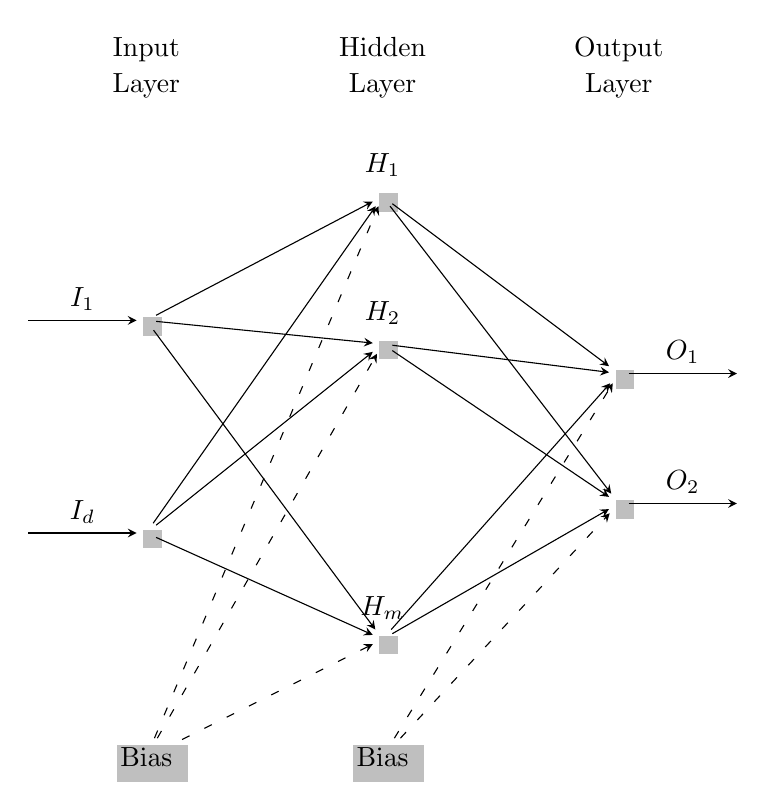
\begin{tikzpicture}[x=1.5cm, y=1.5cm, >=stealth]
%      \foreach \m/\l [count=\y] in {1,missing,2}
%        \node [every neuron/.try, neuron \m/.try, drop shadow] (input-\m) at (0,1.1-\y*0.9) {};
      \node [every neuron/.try, neuron 1/.try, drop shadow] (input-1) at (0,1.1-1*0.9) {};
      \node [every neuron/.try, neuron missing/.try] (input-missing) at (0,1.1-2*0.9) {};
      \node [every neuron/.try, neuron 2/.try, drop shadow] (input-2) at (0,1.1-3*0.9) {};
            
      %\foreach \m [count=\y] in {1,2,missing,3}
      %  \node [neuron hidden/.try, neuron \m/.try ] (hidden-\m) at (2,2.5-\y*1.25) {};
      \node [neuron hidden/.try, neuron 1/.try, drop shadow] (hidden-1) at (2,2.5-1*1.25) {};
      \node [neuron hidden/.try, neuron 2/.try, drop shadow] (hidden-2) at (2,2.5-2*1.25) {};
      \node [every neuron/.try, neuron missing/.try] (hidden-missing) at (2,2.5-2.95*1.25) {};
      \node [neuron hidden/.try, neuron 3/.try, drop shadow] (hidden-3) at (2,2.5-4*1.25) {};
      
      \foreach \m [count=\y] in {1,2}
        \node [neuron output/.try, neuron \m/.try, drop shadow] (output-\m) at (4,0.85-\y*1.1) {};
      
      \foreach \m [count=\y] in {1,2}{
        \node [neuron filled/.try, drop shadow] (bias-\m) at (-2+2*\y,-3.5) {Bias};
      }
      
      % Add the labels to the nodes
      \foreach \l [count=\i] in {1,d}
        \draw [<-] (input-\i) -- ++(-1,0)
        node [above, midway] {$I_\l$};
      
      \foreach \l [count=\i] in {1,2,m}
        \node [above] at (hidden-\i.north) {$H_\l$};
      
      \foreach \l [count=\i] in {1,2}
        \draw [->] (output-\i) -- ++(1,0)
        node [above, midway] {$O_\l$};
      
      % Draw the connecting arrows
      \foreach \i in {1,...,2}
        \foreach \j in {1,...,3}
          \draw [->] (input-\i) -- (hidden-\j);
      
      \foreach \i in {1,...,3}
        \foreach \j in {1,...,2}
          \draw [->] (hidden-\i) -- (output-\j);

      \foreach \i in {1,...,3}
        \draw [loosely dashed, ->] (bias-1) -- (hidden-\i);
      \foreach \i in {1,...,2}
        \draw [loosely dashed, ->] (bias-2) -- (output-\i);
          
      
      \foreach \l [count=\x from 0] in {Input, Hidden, Output}
      \node [align=center, above] at (\x*2,2) {\l \\ Layer};
    \end{tikzpicture} 
    \caption{Base Structure of Our Feed-Forward Network}\label{fig:feedForwardNet}
  \end{figure}
  
  The final structure of our feed forward network is shown in Figure~\ref{fig:feedForwardNet}.  The number of input nodes is dictated by the number of rows in the embedding matrix; as mentioned in Section~\ref{sec:embeddingMatrix}, we used a rank of~$d=25$ in our experiments.  Our sole hidden layer has $m=256$ fully-connected neurons. There are two output nodes (e.g., one for ``Donald Trump'' and the other for ``Hillary Clinton'').  A softmax function normalizes the output probabilities to ensure they sum to probability~$1$.  We selected this paradigm as it simplified the Tensor Flow implementation without affecting the quality of the results.
  
  Our final feed-forward network design used the rectified linear and sigmoid activation functions for the hidden and output layers respectively.  Each neuron in the network also had its own bias input.
  
  \section{Experimental Results} \label{sec:experimentalResults}
  
  As of the writing of this document, our team is ranked sixth in the Kaggle competition with a minimum error of approximately~0.2. This section discusses only those that comply with the minimum requirements of the assignment.  Additional and extra credit experiments are discussed in Sections~\ref{sec:bagOfWords},~\ref{sec:extraNnExperiments}, and~\ref{sec:openSourceWordModels}.
  
  LSTMs can have a greater tendency to overfit than most simple feed forward networks.  We observed this capability to poorly generalize on this dataset where we could get log loss training errors of approximately~$0.05$, but test errors of~$0.7$,~i.e. an increase of more than a order of magnitude.  This overfitting was not due to excessive epochs.  Rather these large divergences could be observed in fewer than 100~full batch trainings.  Even when we did mini-batches, we did not see a significant decrease in the generalization error.
  
  In our experience, LSTMs can be significantly more sensitive to variations in their hyperparameters than simple fully connected feed forward networks.  With our optimal configuration, we were able to achieve a minimum log-loss test error of approximately~\textbf{0.3} with the LSTM.  This required the use of an open-source word model as described in Section~\ref{sec:openSourceWordModels}.  Using a trained embedding matrix, our optimal score was~{0.38}. Overall, we expect that with a larger team and more time, we could have achieved results similar to some of the other teams.
    
  \section{Extra Credit \#1: Bag of Words Model}\label{sec:bagOfWords}
    
  In the ``bag of words'' model, each textual input, i.e., tweet, is transformed into an unordered set of words.  Hence, the contextual and word ordering information is discarded.  This approach removes any sequential relation in the data; hence, the LSTM added no specific value for training.  Hence, we removed the LSTM when performing this experiment and instead trained with just the embedding matrix and the feed-forward network. 
  
  Using the previously described neural-network structure, we were able to get 100\%~accuracy on the complete training set.  Likewise, we get an best-case test set of~\textbf{0.20070} using this approach.
  
  \section{Extra Credit \#2: Neural Network Experiments}\label{sec:extraNnExperiments}
  
  Below are additional experiments we tried beyond the base requirements.  
  
  \subsection{Extra Credit \#2a: Hidden Layer Activation Functions}
  
  We experimented with three activation configurations for the hidden layer.  In addition to rectified linear, we also tried a ``pass-through'' activation where the neuron's output was simply~$\textbf{w}\cdot\textbf{x} + b$, where $\textbf{w}$~is the weight vector, $\textbf{x}$~the input, and $b$~the bias term.  We also tried to use a sigmoid function.  However, these two other activation functions took more epochs to converge (an increase of approximately 200 to 1,000~training rounds) and yield worse testing error.
  
  \subsection{Extra Credit \#2b: Additional Neurons in the Hidden Layer}\label{sec:ecMoreHiddenLayerNeurons}
  
  This is a general (but not strict) correlation between the number of neurons in the hidden layer and the complexity of the function the network can learn.  Additional neurons also increase the possibility of overfitting.  We experiment with three different quantities of hidden layer neurons, namely $128$, $256$, and $512$.  We observed that $128$ and $512$ neurons had similarly poor performance of approximately~$\textbf{0.24}$ on the test set.  In addition, $512$ neurons significantly increased the training time (by a factor of two times).  In contrast, $256$~hidden layer neurons had a training error of~$\sim0.20$, that is why we selected~$d=256$ as discussed in Section~\ref{sec:neuralNetOverview}.
     
  \subsection{Extra Credit \#2c: Multiple Feed-Forward Hidden Layers}
  
  As illustrated in Figure~\ref{fig:feedForwardNet}, our feed-forward network only had a single-hidden layer.  We settled this architecture after experimenting with both two and three hidden layers.  Similar to the findings in Section~\ref{sec:ecMoreHiddenLayerNeurons}, increasing the complexity of the feed-forward network by adding more layers had a dual deleterious effect by both increasing the training time and reducing the reported score on the test set.
     
     
  \subsection{Extra Credit \#2d: Optimizer Selection}
  
  TensorFlow optimizers control the calculation of error gradients and application of these gradients to variables.  TensorFlow includes a suit of different optimizers, which each implementing a different learning algorithm, including: \texttt{AdamOptimizer} (Adaptive Moment Estimation), \texttt{GradientDescentOptimizer} (Stochastic Gradient Descent), \texttt{Adagradoptimizer} (Adaptive Gradient), \texttt{MomentumOptimizer} (Momentum Method), etc.  
  
  As mentioned in Section~\ref{sec:experimentalResults}, tuning the learning rates for an LSTM can be challenging.  Likewise, different optimizers may require hyperparameters that are mutually exclusive to function properly.  In all our experiments, the \texttt{AdamOptimizer} significantly outperformed all other optimizers.  It converged faster and with lower loss on the training set than all the others.  The improvement it provided in training logistic loss could be as high as~\textbf{0.5}.  
  
  \section{Extra Credit \#3: Use of Open-Source Word Models}\label{sec:openSourceWordModels}
  
  Figure~\ref{fig:completeLstmClassifer} shows how an embedding matrix is due to reduce the dimension of the input and to improve learning performance.  Rather than having our neural network learn an embedding matrix solely on its own, an alternative is to use public embedding matrices.  The benefits of this approach include: significantly larger training set, improved embedding matrix coverage for on words that appear only in the test set, etc.  For example, the Google news word model, which we used, contains over three million words and was trained on more than 100~billion words.  In contrast, the tweets in this homework contained only about 11,000~words.
  
  By switching to Google's word model, we saw a log loss improvement of approximately~0.2.
\end{document}